\documentclass{standalone}
\usepackage{kpfonts-otf}
\usepackage{tikz}
\usetikzlibrary{math, patterns}
\usepackage{tkz-euclide}
\usepackage{siunitx}
\begin{document}
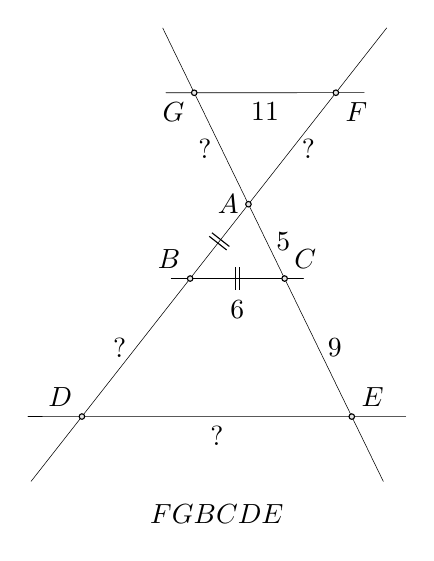
\begin{tikzpicture}[scale=0.15]
    \tkzDefPoint(0,0){B}
    \tkzDefPoint(8,0){C}
    \tkzInterCC[R](B,8 cm)(C,7 cm)\tkzGetPoints{A}{P_2}
    \tkzInterLC[R](A,C)(A, 20 cm)\tkzGetPoints{E_1}{E}
    \tkzDefLine[parallel=through E](C,B)\tkzGetPoint{X}
    \tkzInterLL(E,X)(A,B)\tkzGetPoint{D}
    \tkzInterLC[R](A,B)(A,12 cm)\tkzGetPoints{F}{G_2}
    \tkzDefLine[parallel=through F](C,B)\tkzGetPoint{X}
    \tkzInterLL(F,X)(A,E)\tkzGetPoint{G}
    \tkzLabelPoints[above left](D,B)
    \tkzLabelPoints[above right](E,C)
    \tkzLabelPoints[left](A)
    \tkzLabelPoints[below left](G)
    \tkzLabelPoints[below right](F)
    \tkzDrawLines(D,E B,C G,F)
    \tkzDrawLines(D,F G,E)
    \tkzMarkSegments[mark=||](B,C B,A)
    \tkzLabelSegment[below=1ex](B,C){$6$}
    \tkzLabelSegment[right](A,C){$5$}
    \tkzLabelSegment[right](C,E){$9$}
    \tkzLabelSegment(G,F){$11$}
    \tkzLabelSegment[below=1cm](D,E){$FG \parallele BC \parallele DE$}
    \tkzLabelSegment[left](G,A){?}
    \tkzLabelSegment[left](D,B){?}
    \tkzLabelSegment[right](F,A){?}
    \tkzLabelSegment[below](D,E){?}
    \tkzDrawPoints(B,C,A,E,D,F,G)
    \end{tikzpicture}
\end{document}
